\documentclass[conference]{IEEEtran}

\usepackage{amsmath,amssymb,amsfonts}
\usepackage{algorithm}
\usepackage{algpseudocode}
\usepackage{xcolor}
\usepackage{graphicx}
\usepackage{textcomp}
\usepackage{multirow}
\usepackage{mathtools}
\usepackage{commath}
\usepackage{subcaption}
\usepackage[super]{nth}
\usepackage[style=numeric, backend=bibtex, language=english, maxbibnames=99]{biblatex}

% tikz
\usepackage{tikz}
\usetikzlibrary{shapes.geometric, arrows}
% tikz styles
\tikzstyle{user} = [circle, thick, draw, minimum size=2.5cm]
\tikzstyle{item} = [rectangle, thick, draw, minimum width=3cm, minimum height=1.5cm]
\tikzstyle{arrow} = [->, draw, thick]
\tikzstyle{bi-arrow} = [<->, draw, thick]
\tikzstyle{line} = [-, draw, thick]

\def\BibTeX{{\rm B\kern-.05em{\sc i\kern-.025em b}\kern-.08em
    T\kern-.1667em\lower.7ex\hbox{E}\kern-.125emX}}

\emergencystretch=8em

\bibliography{literature}

\begin{document}

\title{Community Embeddings for Friend Suggestions}

\author{
    \IEEEauthorblockN{Anton I. N. Begehr}
    \IEEEauthorblockA{
        \textit{Graduate School of Business}\\
        \textit{National Research University Higher School of Economics}\\
        Moscow, Russia\\
        a.begehr@fu-berlin.de\\
    }
    \and
    \IEEEauthorblockN{Prof. Dr. Petr Panfilov}
    \IEEEauthorblockA{
        \textit{Graduate School of Business}\\
        \textit{National Research University Higher School of Economics}\\
        Moscow, Russia\\
        ppanfilov@hse.ru\\
    }
}

\maketitle

\begin{abstract}
    Graphs, such as social networks, emerge naturally from various real-world situations. Recently, graph embedding methods have gained traction in data science research.
    Recommender systems are used in a wide range of business applications and are essential for online, e-business models to survive and strive in the contemporary market. Using graph embeddings for recommendation tasks, have the possibility of improving upon recommender systems, because of data compression, their feature vector format, and sub-quadratic time complexity.
    Graph and community embeddings generated with ComE BGMM+VI are used to build a recommender system for friend suggestions. ComE BGMM+VI is an alteration of the community embeddings algorithm ComE. ComE BGMM+VI applies a Bayesian Gaussian mixture model and variational inference for community embedding and detection.
    Recommendations are evaluated by the top-N hit-rate over users with at least 50 friends. A friend suggestions recommender system with a top-10 leave-one-out hit-rate of 43.6\% and run-time optimized 32.9\% is presented.
\end{abstract}

\begin{IEEEkeywords}
    graph, embedding, community embedding, ComE, recommendations, friend suggestions
\end{IEEEkeywords}


\section{Introduction}

Graphs, such as social networks, knowledge graphs, content-rating graphs, and communication networks, emerge naturally from various real-world situations. Analyzing these graphs leads to findings and understanding of the underlying structures, coherences, and dependencies. Recently, methods for embedding graph's nodes into lower-dimensional Euclidean spaces, called graph embeddings, have gained traction in multiple areas of data science research \cite{Goyal_2018}.

Due to the rapid growth of the internet and data accumulation, recommender systems are essential for e-business and online business models to survive and strive in the contemporary market \cite{Polatidis2013RecommenderST}. Modern recommender systems need to take into account the huge amounts of user data generated at all times in big data systems around the world and improve recommendations instead of failing under the thrust of big data overload.

Utilizing graph embeddings for recommendation tasks, has recently gained research traction \cite{Palumbo2018AnEC, Palumbo2018KnowledgeGE, GradGyenge2017GraphEB, Sathish2019GraphEB}. The advantages of graph embeddings include data compression and the Euclidean feature vector format \cite{Godec2018}. Given these advantages and provided competitive results, graph embeddings have the possibility of greatly improving upon graph-based use-cases like recommender systems.

Community Embeddings, in addition to embedding a graph's nodes through first- and second-order proximity, also preserve higher-order proximity by embedding clusters present in the graph data. The graph and community embedding algorithm ComE aims to preserve first-, second- and higher-order proximity by embedding a graph's nodes and communities \cite{ComE}.

This work specifically examines community embeddings for friend suggestion recommender systems and evaluates recommendations on social network graph data for the use-case of friend suggestions. Graph and community embeddings generated with ComE BGMM+VI are used to develop a friend suggestions recommender system based on the shortest distances between nodes in the embedding. Recommendations are evaluated by the top-$N$ recommendations hit-rate of test edges. A friend suggestions recommender system with a top-10 leave-one-out hit-rate of 43.6\% and run-time optimized 32.9\% is presented.

\begin{figure}[h]
    \centering
    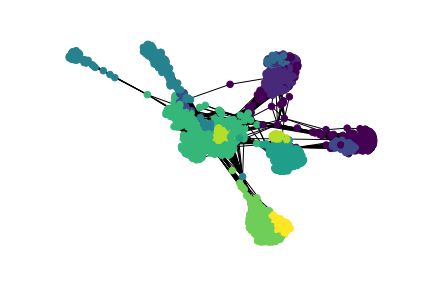
\includegraphics[width=0.48\textwidth]{images/fb/graph_d4.png}
    \caption{\citetitle{social_circles_fb} graph plotted with networkx's spring layout and node colors representing community membership obtained by ComE BGMM+VI with $D=4$.\cite{networkx}}
    \label{fig:fb_graph}
\end{figure}


\section{Friend Suggestions}

Recommender Systems are eagerly researched in academia and widely deployed in real-world business applications. Most contemporary technology companies heavily rely on recommender systems to drive usage of their services and consumption of their content. Users, in turn, rely on recommender systems to find what they want and need and save searching time. State-of-the-art recommender systems provide a competitive advantage desperately needed by online services. Companies heavily relying on recommender systems include YouTube, Amazon, Netflix, and many more \cite{Rocca19}.

Recommender systems are built on top of user-item interaction. Friend suggestions are a simpler type of recommender system. For friend suggestions, no distinction is made between users and items. The entity user is both the subject and object of recommendation. This results in a simple data model, which can be used for structural friend suggestions, as shown in Fig. \ref{fig:data_model}.

\begin{figure}[h]
    \centering
    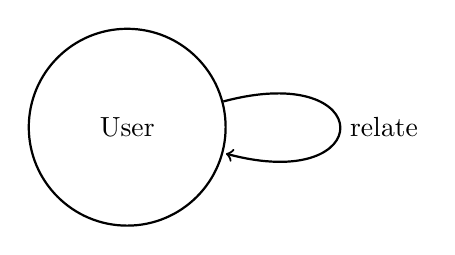
\begin{tikzpicture}[node distance=6cm]
        \node (user) [user] {User};
        \path [arrow] (user) edge[loop right] node[right]{relate} (user);
    \end{tikzpicture}
    \caption{Minimal data model supporting friend suggestions.}
    \label{fig:data_model}
\end{figure}

The two main methods used for recommender systems are collaborative filtering and content-based filtering. Collaborative filtering is based on the assumption that users like items similar to other items they like and items that are liked by other users with similar tastes \cite{Grover17, Su2009ASO}. Content-based filtering considers user and item attributes, instead of solely interactions \cite{Rocca19, Lops2011SurveyCB}.

In this paper, a method of generating friend suggestions based solely on graph data structure, and not on the node or edge attributes, is presented. The graph of users and friendships is embedded to a lower-dimensional space with the community embedding algorithm ComE BGMM+VI \cite{ComE, ComE+, ComE_BGMM_GH}. The approach can be considered a variant of collaborative filtering with the euclidean distance of user embeddings and user community membership as measures for user similarity. The proposed advantage of using such an approach is that community embeddings optimize first-, second-, and higher-order proximity between users in the node embedding.

\subsection{Evaluation}

To determine the effectivity of friend suggestions, the generated friend suggestions must be properly validated. In this paper, the top-$N$ approach to evaluating recommender systems with hit-rate as the evaluation metric is chosen.

A user's top-$N$ recommendations is a list of $N$ items to be recommended to a specific user. To evaluate recommender systems with the top-$N$ and hit-rate approach, initially, the dataset is split into train and test data. For each testing user, one relation is left out, according to the leave-one-out method and the model is trained on the remaining training dataset. Once the model is trained, a list of top-$N$ recommendations is generated for each testing user. If the item corresponding to the user is in the user's top-$N$ list, a hit is counted, otherwise, a miss is counted. The hit-rate is defined as the total number of hits divided by the number of testing users.

Utilizing the top-$N$ approach with hit-rate to evaluate recommender systems is advantageous to evaluating recommender systems by a link prediction approach since the top-$N$ approach is more realistic in comparison to actual recommender system use-cases. When you open Netflix, Amazon, YouTube, or Facebook friend suggestions, one or multiple top-$N$ recommendation lists are generated and displayed. If you click on an item and buy, watch, or befriend, that is considered a hit, otherwise, a miss.

The hit-rate metric on top-$N$ recommendations provides a realistic option of evaluating recommender systems and with the leave-one-out (LOO) strategy is used often in literature \cite{Cremonesi2010PerformanceOR, Palumbo2017entity2rec, Zhao2019ATS, He2017NeuralCF}.


\section{Algorithm}

The proposed algorithm for generating friend suggestions using community embeddings is detailed and evaluated on time complexity. The initially quadratic runtime of generating friend suggestions for all users is then reduced by a factor of $K$ by utilizing a node's community membership. The two resulting algorithms are presented.

Algorithm \ref{alg:friend_sug} describes in pseudocode how recommendations are computed from node embeddings generated by ComE BGMM+VI. The terms friend suggestions and social recommendations are used interchangeably.

\begin{algorithm}
    \caption{Top-$N$ Social Recommendations based on Node Embeddings}
    \label{alg:friend_sug}
    \begin{algorithmic}[1]
        \Require{graph $G = (V, E)$, maximum number of communities K, number of walks $\gamma$, walk length $\ell$, window size $\zeta$, representation size $D$, negative context size $m$, parameters ($\alpha$, $\beta$), number of recommendations $N$.}
        \Ensure{Top-$N$ recommendations for all nodes $R$.}
        % run ComE BGMM+VI
        \State $\Phi, \Phi', \Pi, (\Psi,\Sigma) \leftarrow ComE(G, K, \gamma, \ell, \zeta, D, m, \alpha, \beta)$
        % find friends
        \For{$(v, v') \in E$}
        \State $F_v \leftarrow F_v \cup \{v'\}$
        \State $F_{v'} \leftarrow F_{v'} \cup \{v\}$
        \EndFor
        % for each node
        \For{$v \in V$}
        % generate ascending recommendation list for each node
        \State $R_v \leftarrow SortedDict(size=N)$
        \For{$v' \in V \land v' \notin F_v \land v' \neq v$}
        \State $d \leftarrow \|\phi_v - \phi_{v'}\|$
        \State $R_v[d] \leftarrow v'$
        \EndFor
        % get Top-N recommendations for each node
        \State $R_v  \leftarrow R_v.values()$
        \EndFor
    \end{algorithmic}
\end{algorithm}

The function $ComE(G, K, \gamma, \ell, \zeta, D, m, \alpha, \beta)$ is the ComE BGMM+VI community embedding algorithm. It returns the node embedding $\Phi$, context embedding $\Phi'$, community assignment $\Pi$, and community embedding $(\Psi,\Sigma)$. ComE BGMM+VI is based on the ComE algorithm presented by \citeauthor{ComE} in their paper \citetitle{ComE} as algorithm 1 on page 381 of the publication's in-proceeding \cite{ComE}. ComE BGMM+VI takes a Bayesian approach to community embedding by utilizing  a Bayesian Gaussian mixture model (BGMM) and variational inference (VI) for community embedding and detection instead of a non-Bayesian Gaussian mixture model (GMM) with expectation maximization (EM) \cite{ComE_BGMM_GH}. %TODO citation to the ComE BGMM paper.

The runtime of ComE BGMM+VI is equivalent to the runtime of ComE in its big-$O$ notation. ComE's time complexity is $O(\abs{V}\gamma\ell + \abs{V} + T_1 (T_2\abs{V}K + K + \abs{E} + \abs{V}\gamma\ell + \abs{V}K))$, which is linear in time complexity to the graph size: $O(\abs{V} + \abs{E})$ (line 1) \cite{ComE}. All friends of each user are determined in $O(E)$ (lines 2-5). A sorted dictionary of the top-$N$ friend suggestions for each user sorted ascending by distances between the node embeddings is computed in $O(\abs{V}^2N))$ (lines 6-13). Top-$N$ friend suggestions are generated for each user: $O(\abs{V})$. For each user, all users not befriended currently are considered ($O(\abs{V})$) and inserted into a sorted dictionary of length $N$ ($O(N)$).

This brings the total time complexity of Algorithm \ref{alg:friend_sug} to $O(\abs{V}\gamma\ell + \abs{V} + T_1 (T_2\abs{V}K + K + \abs{E} + \abs{V}\gamma\ell + \abs{V}K) + \abs{E} + \abs{V}^2N)$. We consider $\gamma$, $\ell$, $T_1$, $T_2$, and $N$ as constant, therefore the time complexity depends on the graph's size $(\abs{V}, \abs{E})$ and the number of communities $K$: $O(K + \abs{V}K + \abs{E} + \abs{V}^2)$.

Algorithm \ref{alg:friend_sug_com} describes in pseudocode how recommendations are computed from ComE BGMM+VI node and community embeddings and community assignments. The advantage of also considers community membership, is that an improvement in time complexity can be obtained, by considering only users in the same community for friend suggestions.

\begin{algorithm}
    \caption{Top-$N$ Social Recommendations based on Node and Community Embeddings}
    \label{alg:friend_sug_com}
    \begin{algorithmic}[1]
        \Require{graph $G = (V, E)$, maximum number of communities K, number of walks $\gamma$, walk length $\ell$, window size $\zeta$, representation size $D$, negative context size $m$, parameters ($\alpha$, $\beta$), number of recommendations $N$.}
        \Ensure{Top-$N$ recommendations for all nodes $R$.}
        % run ComE BGMM+VI
        \State $\Phi, \Phi', \Pi, (\Psi,\Sigma) \leftarrow ComE(G, K, \gamma, \ell, \zeta, D, m, \alpha, \beta)$
        %  generate a set of nodes for each community
        \For{$v \in V$}
        \State $k \leftarrow \pi_v$
        \State $C_k \leftarrow C_k \cup \{v\}$
        \EndFor
        % find friends
        \For{$(v, v') \in E$}
        \State $F_v \leftarrow F_v \cup \{v'\}$
        \State $F_{v'} \leftarrow F_{v'} \cup \{v\}$
        \EndFor
        % for each node
        \For{$v \in V$}
        % generate ascending recommendation list for each node
        \State $R_v \leftarrow SortedDict(size=N)$
        \For{$v' \in C_k \land v' \notin F_v \land v' \neq v$}
        \State $d \leftarrow \|\phi_v - \phi_{v'}\|$
        \State $R_v[d] \leftarrow v'$
        \EndFor
        % get Top-N recommendations for each node
        \State $R_v  \leftarrow R_v.values()$
        \EndFor
    \end{algorithmic}
\end{algorithm}

Line 1, lines 6-9, and lines 10-17, except for line 12, are the same in Algorithm \ref{alg:friend_sug_com} as in Algorithm \ref{alg:friend_sug}. All users are filtered into sets $C_k$, one for each community $k$ in $O(\abs{V})$ (lines 2-5). Instead of considering the set of all non-friends users of size $\abs{V}$, only users in the same community $C_k$ of size $\frac{\abs{V}}{K}$ are considered (line 12) in $O(\frac{\abs{V}^2N}{K})$.

This brings the total time complexity of Algorithm \ref{alg:friend_sug_com} to $O(\abs{V}\gamma\ell + \abs{V} + T_1 (T_2\abs{V}K + K + \abs{E} + \abs{V}\gamma\ell + \abs{V}K) + \abs{V} + \abs{E} + \frac{\abs{V}^2N}{K})$. Again, we consider $\gamma$, $\ell$, $T_1$, $T_2$, and $N$ as constant, therefore the time complexity depends on the graph's size $(\abs{V}, \abs{E})$ and the number of communities $K$: $O(K + \abs{V}K + \abs{E} + \frac{\abs{V}^2}{K})$.

The runtimes for Algorithm \ref{alg:friend_sug} and \ref{alg:friend_sug_com} when considering $K$ as constant or scaling w.r.t the graph $G = (V, E)$ are shown in Table \ref{tab:runtimes}. The number of friend suggestions $N$ is considered constant w.r.t the graph $G = (V, E)$.

\begin{table}
    \centering
    \caption{Algorithm \ref{alg:friend_sug} and \ref{alg:friend_sug_com} time complexity.}
    \label{tab:runtimes}
    \begin{tabular}{l l | c}
        \multirow{2}{*}{$K$ constant} & Algorithm \ref{alg:friend_sug}     & $O(\abs{E} + \abs{V}^2)$                          \\
                                      & Algorithm \ref{alg:friend_sug_com} & $O(\abs{E} + \abs{V}^2)$                          \\
        \hline
        \multirow{2}{*}{$K$ scaling}  & Algorithm \ref{alg:friend_sug}     & $O(K + \abs{V}K + \abs{E} + \abs{V}^2)$           \\
                                      & Algorithm \ref{alg:friend_sug_com} & $O(K + \abs{V}K + \abs{E} + \frac{\abs{V}^2}{K})$ \\
    \end{tabular}
\end{table}

When the hyperparameter number of communities $K$ is considered non-constant with respect to the graph $G$, Algorithm \ref{alg:friend_sug_com} reduces the quadratic runtime in comparison to Algorithm \ref{alg:friend_sug_com}.
$K$ can therefore reduce the quadratic summand $\abs{V}^2N$ by only considering users of the same community for friend suggestions. The reduction in time complexity through Algorithm \ref{alg:friend_sug_com} is only scalable when considering $K$ to be scale with the input graph's size. This assumption can be made when considering communities as groups of friends: with ten times more users, these users form ten times more communities.


\section{Visual Example}

The small \citetitle{KarateClubDS} dataset will be used to visually underline the motivation for using node embedding and community memberships generated by ComE BGMM+VI for generating friend suggestions for person nodes on the karate club graph \cite{KarateClubDS}.

\begin{figure}[h]
    \centering
    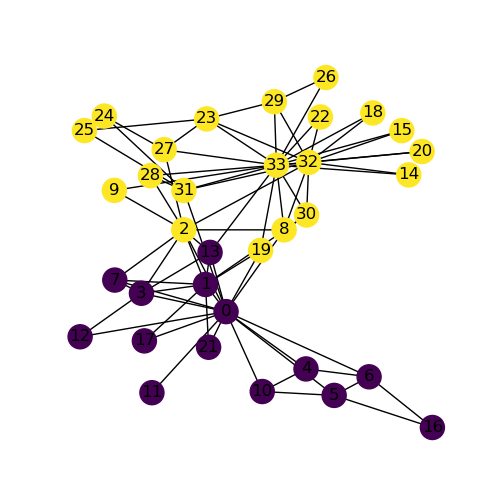
\includegraphics[width=0.4\textwidth]{images/karateclub/spring.png}
    \caption{\citetitle{KarateClubDS} plotted with networkx's spring layout \cite{KarateClubDS, networkx}.}
    \label{fig:karateclub_spring}
\end{figure}

Fig. \ref{fig:karateclub_spring} shows the 34 nodes and 78 edges of the \citetitle{KarateClubDS} dataset plotted as a graph with the Python network package networkx's spring layout.\cite{networkx} Spring layout simulates a force-directed representation of the network, by treating edges as springs pulling nodes together and treating nodes as repelling objects, sometimes called an anti-gravity force.\cite{networkx} The node classification, represented by node color, shown in Fig. \ref{fig:karateclub_spring} was obtained by running ComE with BGMM and VI with the hyperparameters presented in Table \ref{tab:params_karateclub}.

\begin{table}
    \centering
    \caption{Hyperparameters used for the Karateclub dataset.}
    \label{tab:params_karateclub}
    \begin{tabular}{ l | c | r }
        parameter                    & notation & value     \\
        \hline
        \hline
        number\_walks                & $\gamma$ & $10$      \\
        \hline
        walk\_length                 & $\ell$   & $80$      \\
        \hline
        representation\_size         & $D$      & $2$       \\
        \hline
        num\_workers                 & \empty   & $10$      \\
        \hline
        num\_iter                    & \empty   & $3$       \\
        \hline
        reg\_covar                   & \empty   & $0.00001$ \\
        \hline
        batch\_size                  & \empty   & $50$      \\
        \hline
        window\_size                 & $\zeta$  & $10$      \\
        \hline
        negative                     & $m$      & $5$       \\
        \hline
        lr                           & \empty   & $0.025$   \\
        \hline
        alpha                        & $\alpha$ & $0.1$     \\
        \hline
        beta                         & $\beta$  & $0.1$     \\
        \hline
        down\_sampling               & \empty   & $0.0$     \\
        \hline
        communities                  & $K$      & $5$       \\
        \hline
        weight\_concentration\_prior & $\Gamma$ & $10^{-5}$ \\
    \end{tabular}
\end{table}

As can be seen in Figure \ref{fig:karateclub_spring}, the two communities in the \citetitle{KarateClubDS} dataset are correctly identified, despite the number of communities being initialized with $K=5$. Thanks to the Bayesian approach to community modeling and optimization through variational inference, three unused communities are dropped, which leaves the prominent two communities present in the dataset. The node classification obtained reflects the node classification published in the \citeyear{ComE} original ComE paper by \citeauthor{ComE}.\cite{ComE}

\subsection{Training and Testing Split}

\citetitle{KarateClubDS} is split into training and testing parts. For evaluation, the leave-one-out (LOO) method is used, where for each testing user one edge is left out, then if the left out edge is in the user's top-$N$ recommendations, a hit is counted, otherwise, a miss is recorded.

The three users with the highest degree are chosen as testing users: user 30, user 0, and user 32. For each testing user, a LOO-testing edge is chosen: (30, 23), (0, 1), and (32, 30). These three testing edges are spared for the testing dataset and omitted from the training graph.

\subsection{Embedding}

ComE BGMM+VI is run with the hyperparameters listed in Table \ref{tab:params_karateclub} on the training dataset. The resulting node and community embeddings are visualized as node embeddings colored by community membership and community embeddings plotted as ellipses in Fig. \ref{fig:karateclub_emb}.

\begin{figure}[h]
    \centering
    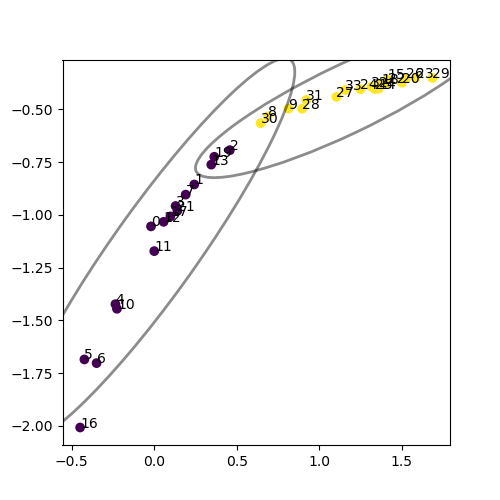
\includegraphics[width=1\linewidth]{images/karateclub/embeddings_5.png}
    \caption{\citetitle{KarateClubDS} training dataset node and community embedding and node classification.}
    \label{fig:karateclub_emb}
\end{figure}

\subsection{Friend Suggesting}

With embeddings generated, top-$N$ friend suggestion recommendations are generated from the training node and community embeddings for the testing users. For each testing user, a ranked list of non-friend users from the same community is generated (Algorithm \ref{alg:friend_sug_com}). A test user's friend suggestion list is ordered in ascending order by the euclidean distance between the node embeddings. Table \ref{tab:karateclub_emb_dists} shows the test users' friend suggestion ranked lists.

\begin{table}
    \centering
    \caption{Testing users' friend suggestions ranked by node embedding distance.}
    \label{tab:karateclub_emb_dists}
    \begin{subfigure}{.4\textwidth}
        \centering
        \begin{tabular}{ c | r }
            User        & Distance   \\
            \hline
            \hline
            24          & $0.137181$ \\
            \hline
            25          & $0.214332$ \\
            \hline
            \textbf{23} & $0.543287$ \\
        \end{tabular}
        \caption{user 33}
    \end{subfigure}
    \begin{subfigure}{.4\textwidth}
        \centering
        \begin{tabular}{ c | r }
            User       & Distance   \\
            \hline
            \hline
            \textbf{1} & $0.322270$ \\
            \hline
            16         & $1.030336$ \\
        \end{tabular}
        \caption{user 0}
    \end{subfigure}
    \begin{subfigure}{.4\textwidth}
        \centering
        \begin{tabular}{ c | r }
            User        & Distance   \\
            \hline
            \hline
            25          & $0.039816$ \\
            \hline
            24          & $0.045994$ \\
            \hline
            27          & $0.182484$ \\
            \hline
            26          & $0.255288$ \\
            \hline
            28          & $0.356683$ \\
            \hline
            9           & $0.501317$ \\
            \hline
            \textbf{30} & $0.668306$ \\
        \end{tabular}
        \caption{user 32}
    \end{subfigure}
\end{table}

The testing users' removed edges make it to the lists successfully; therefore, the removed friends are in the same community as the test users and can be recommended through friend suggestions.

\subsection{Evaluation}

The top-$N$ friend suggestions, generated for the testing users with Algorithm \ref{alg:friend_sug_com}, are evaluated against the three removed test edges.
The ranked lists of friend-suggestions shown in Figure \ref{tab:karateclub_emb_dists} is used to determine top-$N$ friend suggestions for each testing user and evaluate the recommendations my the hit-rate metric. The LOO-testing edges are printed bold in Table \ref{tab:karateclub_emb_dists}. The resulting top-$N$ hit-rates are plotted against the number of suggestions $N$ in Fig. \ref{fig:karateclub_hitrates}.

\begin{figure}[h]
    \centering
    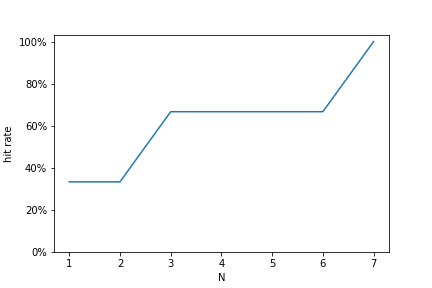
\includegraphics[width=.4\textwidth]{images/karateclub/hit_rates.png}
    \caption{Hit-rates from top-$N$ recommendations on \citetitle{KarateClubDS}.}
    \label{fig:karateclub_hitrates}
\end{figure}

Fig. \ref{fig:karateclub_hitrates} shows promising results for using ComE to generate top-$N$ friend suggestions on the small \citetitle{KarateClubDS}. The achieved hit-rate starts at 33\% for $N=1$, reaches 67\% at $N=3$, and maxes out at 100\% for $N=7$; therefore, when presenting three friend suggestions to one test user, at least in $66\%$ of cases a friend suggestion would be of interest.


\section{Facebook Friend Suggestions}

The recommender system based on community embeddings with the Bayesian Gaussian mixture model and variational inference is quantitatively evaluated. Friend suggestions are generated for the \citetitle{social_circles_fb} dataset \cite{social_circles_fb, social_circles_in_ego_networks}.

The method of generating friend suggestions using ComE BGMM+VI embeddings and the smallest-distance approach is applied to the \citetitle{social_circles_fb} graph. Both Algorithm \ref{alg:friend_sug} and Algorithm \ref{alg:friend_sug_com} are evaluated. The top-$N$ recommendations are evaluated by the hit-rate metric.

\subsection{Dataset}

The \citetitle{social_circles_fb} dataset was sourced from the profile and network data of ten ego-networks (egonets) through a custom Facebook app by \citeauthor{social_circles_in_ego_networks} as part of their \citeyear{social_circles_in_ego_networks} article \citetitle{social_circles_in_ego_networks}.\cite{social_circles_in_ego_networks}

Fig. \ref{fig:egonet} shows an illustration of the ego-network of user $u$. User $u$ has direct connections to $v_i$, called alters. Alters can be connected to each other and build circles of users, like families, high school friends, or college friends.

\begin{figure}[h]
    \centering
    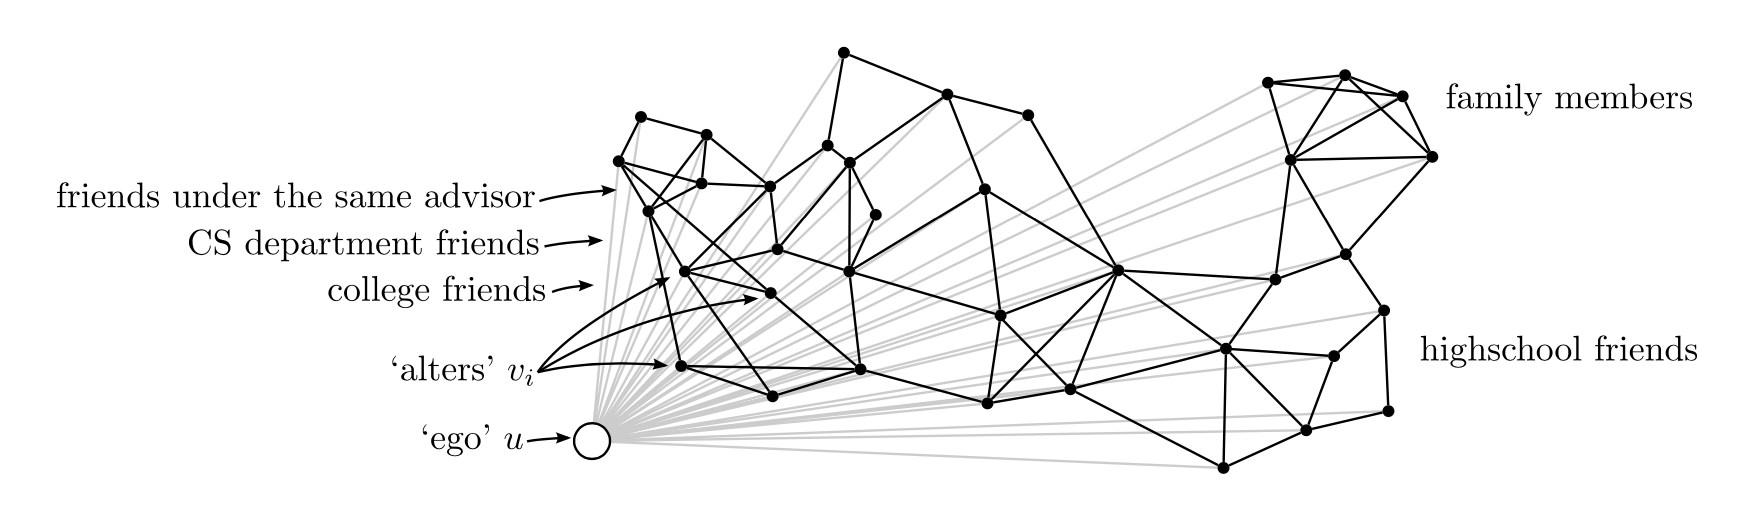
\includegraphics[width=0.48\textwidth]{images/fb/egonet.png}
    \caption{Illustrative example of an ego-network \cite{social_circles_in_ego_networks}.}
    \label{fig:egonet}
\end{figure}

\citeauthor{social_circles_in_ego_networks} obtained profile and network data from ten Facebook ego-networks. The dataset contains 4039 users (nodes) and 88234 friendships (edges).

\subsection{Training and Testing Split}

The \citetitle{social_circles_fb} graph is split into training and testing parts. For evaluation, the leave-one-out (LOO) method is used, where for each testing user one edge is left out, then if the left out edge is in the user's top-$N$ recommendations, a hit is counted, otherwise, a miss is recorded.
Users with only one connection are removed from the dataset since no network information is added by them.

$1169$ of the 4039 users of the \citetitle{social_circles_fb} graph have at least $50$ connections and are used for testing friend suggestions. The threshold of $50$ friends for considering users for testing is set to make sure enough data is available to make sensable suggestions for testing users.

Now that the testing users are identified, the leave-one-out method is employed for obtaining one testing friendship per testing user. The friendship chosen to leave out for testing for each testing user is chosen randomly using NumPy's random choice.\cite{oliphant2006guide, van2011numpy}

\subsection{Embedding}

Community embeddings for the \citetitle{social_circles_fb} graph are generated by running ComE BGMM+VI with the hyperparameters listed in Table \ref{tab:params_fb}.

\begin{table}
    \centering
    \caption{Hyperparameters used for the \citetitle{social_circles_fb} dataset.}
    \label{tab:params_fb}
    \begin{tabular}{ l | c | r }
        parameter                    & notation & value       \\
        \hline
        \hline
        number\_walks                & $\gamma$ & $10$        \\
        \hline
        walk\_length                 & $\ell$   & $80$        \\
        \hline
        representation\_size         & $D$      & $2, 4, 128$ \\
        \hline
        num\_workers                 & \empty   & $10$        \\
        \hline
        num\_iter                    & \empty   & $3$         \\
        \hline
        com\_n\_init                 & \empty   & $10$        \\
        \hline
        reg\_covar                   & \empty   & $0.00001$   \\
        \hline
        batch\_size                  & \empty   & $50$        \\
        \hline
        window\_size                 & $\zeta$  & $10$        \\
        \hline
        negative                     & $m$      & $5$         \\
        \hline
        lr                           & \empty   & $0.025$     \\
        \hline
        alpha                        & $\alpha$ & $0.1$       \\
        \hline
        beta                         & $\beta$  & $0.1$       \\
        \hline
        down\_sampling               & \empty   & $0.0$       \\
        \hline
        communities                  & $K$      & $10$        \\
        \hline
        weight\_concentration\_prior & $\Gamma$ & $10^{-5}$   \\
    \end{tabular}
\end{table}

As is shown in Table \ref{tab:params_fb}, the embedding's representation size $D$ is varied along three values. A representation size $D \in [2,4,128]$ is chosen to determine the effect of the embedding's dimensionality on friend suggestions. It is hypothesized, that two dimensions are not sufficient to capture the structure of the \citetitle{social_circles_fb} graph, due to its size, therefore higher dimensional embeddings are evaluated as well.

Fig. \ref{fig:fb_emb_anim_d2}, Fig. \ref{fig:fb_emb_anim_d4}, and Fig. \ref{fig:fb_emb_anim_d128} show the node embeddings generated by ComE BGMM+VI after one, two, and three iterations. The nodes are colored by community membership from ComE's community embedding and detection.
The $4$- and $128$-dimensional node and community embeddings cannot effectively be plotted in two-dimensional print. Instead, in Figures \ref{fig:fb_emb_anim_d4} and \ref{fig:fb_emb_anim_d128} the two first dimensions of the node and community embeddings are plotted to gain a narrow perspective on the resulting node embeddings.

\newcommand{\fbEmbAnimD}[1]{
    \begin{figure*}[h]
        \centering
        \begin{subfigure}{.33\textwidth}
            \centering
            \includegraphics[width=1\linewidth]{images/fb/anim_d#1_i0.png}
            \caption{\nth{1} Iteration}
        \end{subfigure}%
        %
        \begin{subfigure}{.33\textwidth}
            \centering
            \includegraphics[width=1\linewidth]{images/fb/anim_d#1_i1.png}
            \caption{\nth{2} Iteration}
        \end{subfigure}%
        %
        \begin{subfigure}{.33\textwidth}
            \centering
            \includegraphics[width=1\linewidth]{images/fb/anim_d#1_i2.png}
            \caption{\nth{3} Iteration}
        \end{subfigure}%
        %
        \caption{Node embeddings segment with representation size $D=#1$.}
        \label{fig:fb_emb_anim_d#1}
    \end{figure*}
}

\fbEmbAnimD{2}
\fbEmbAnimD{4}
\fbEmbAnimD{128}

Fig. \ref{fig:fb_graphs} shows the graph spring plotted with networkx and nodes colored by community membership after the lastest iteration of ComE.\cite{networkx} The spring plotted graph structure on Figure \ref{fig:fb_graphs} suggest, that with embedding dimension $D=4$, more fitting communities are detected than for $D=2$ and $D=128$.

\begin{figure*}[h]
    \centering
    \begin{subfigure}{.33\textwidth}
        \centering
        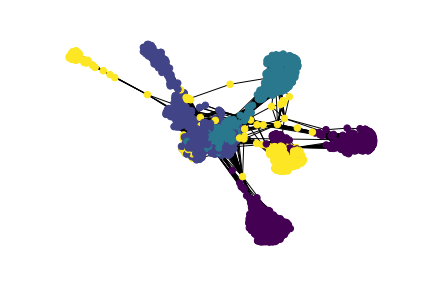
\includegraphics[width=1\linewidth]{images/fb/graph_d2.png}
        \caption{$D=2$}
    \end{subfigure}%
    %
    \begin{subfigure}{.33\textwidth}
        \centering
        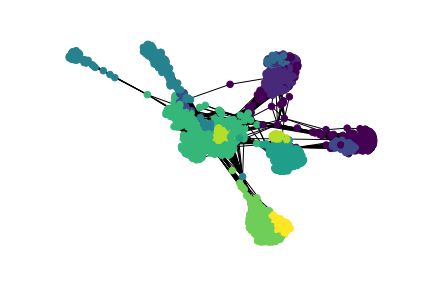
\includegraphics[width=1\linewidth]{images/fb/graph_d4.png}
        \caption{$D=4$}
    \end{subfigure}%
    %
    \begin{subfigure}{.33\textwidth}
        \centering
        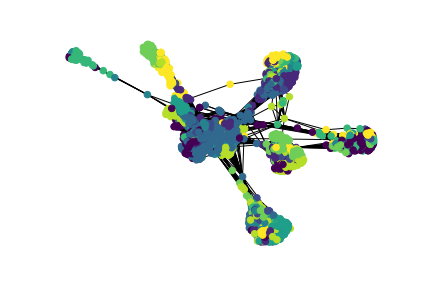
\includegraphics[width=1\linewidth]{images/fb/graph_d128.png}
        \caption{$D=128$}
    \end{subfigure}%
    %
    \caption{Spring plotted graphs with nodes colored by community membership after last ComE BGMM+VI iteration.}
    \label{fig:fb_graphs}
\end{figure*}

Figure \ref{fig:fb_emb_anim_d2} shows node and community embeddings with representation size $D=2$. The limiting two-dimensional space does not allow ComE to represent the \citetitle{social_circles_fb} graph's structure sufficiently to utilize the $K=10$ components of the Gaussian mixture model. Only three components are used after the last of three iterations.

While Figures \ref{fig:fb_emb_anim_d4} and \ref{fig:fb_emb_anim_d128} show only the first two dimensions, of the node embedding of 4 or 128 dimensionality respectively, the general structure of communities is visible. The development of the node embeddings over the three iterations shows the manifestation of the first-, second-, and higher-order proximity by ComE's closed loop. The node embeddings are densified in their communities and spread out in regards to other communities. All $K=10$ components of the Gaussian mixture model are used for $D=4$ and $D=128$.

The nodes are distributed over the $K=10$ communities as shown in the histograms in Figure \ref{fig:fb_emb_weights}. Figure \ref{fig:fb_emb_weights_d2} shows that with representation size $D=2$, ComE BGMM+VI drops 6 communites, effecitvelly using only 4 communities in the final embedding, because the two-dimensional node embeddings are not expressive enough to support more communities. Figures \ref{fig:fb_emb_weights_d4} and \ref{fig:fb_emb_weights_d128} show that with representation sizes $D=4$ and $D=128$ respectivelly, all $K=10$ communities are used.

The tradeoff between the representation size of the embedding $D$ and the embedding expressiveness is demonstrated. When choosing a too low-dimensional embedding, the embedding might not be expressive enough to capture the communities and reduces the quality of the community embedding and detection. When choosing a too high-dimensional embedding, the node embeddings get so expressive that BGMM+VI is not able to drop unused communities because all communities are used in one of the many dimensions.

\begin{figure*}[h]
    \centering
    %
    \begin{subfigure}{.33\textwidth}
        \centering
        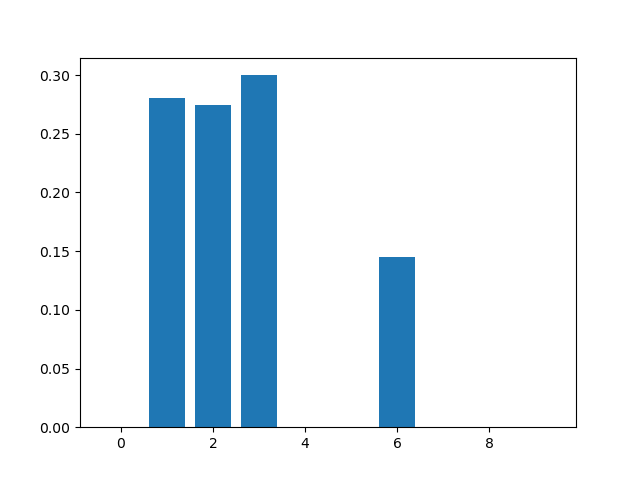
\includegraphics[width=1\linewidth]{images/fb/weights_d2.png}
        \caption{$D=2$}
        \label{fig:fb_emb_weights_d2}
    \end{subfigure}%
    %
    \begin{subfigure}{.33\textwidth}
        \centering
        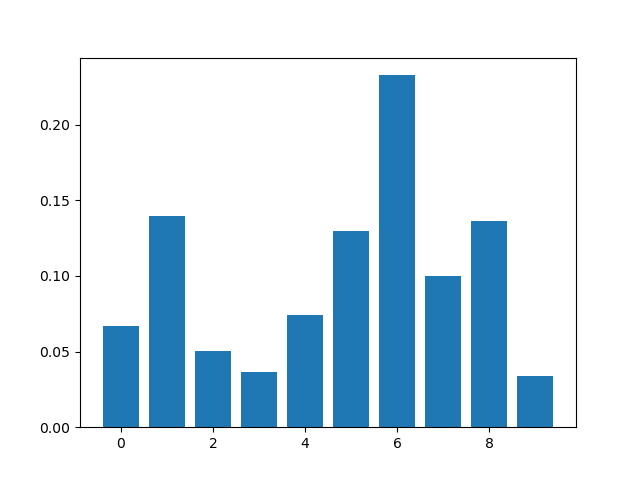
\includegraphics[width=1\linewidth]{images/fb/weights_d4.png}
        \caption{$D=4$}
        \label{fig:fb_emb_weights_d4}
    \end{subfigure}%
    %
    \begin{subfigure}{.33\textwidth}
        \centering
        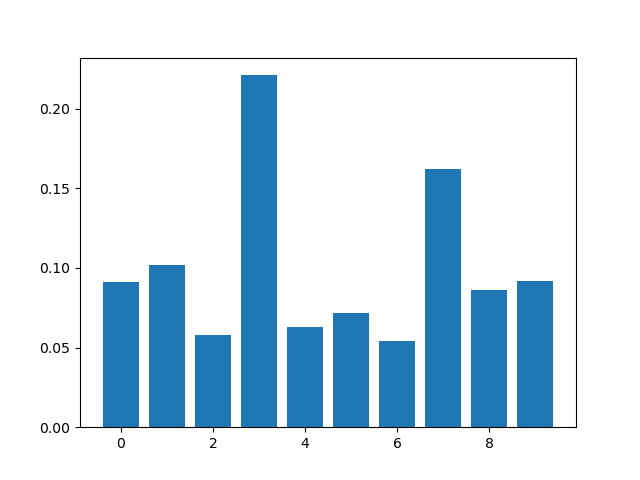
\includegraphics[width=1\linewidth]{images/fb/weights_d128.png}
        \caption{$D=128$}
        \label{fig:fb_emb_weights_d128}
    \end{subfigure}%
    %
    \caption{Weights of communities with $K=10$ and $D \in [2,4,128]$.}
    \label{fig:fb_emb_weights}
\end{figure*}

\subsection{Friend Suggestions}

With node and community embeddings and community assignments generated for $D \in [2,4,128]$ and $K=10$ with training data in the previous section, top-$N$ friend suggestion recommendations are generated from the training node and community embeddings with Algorithm \ref{alg:friend_sug} and Algorithm \ref{alg:friend_sug_com}.

The shortest-embeddings-distance approach is employed, recommending friends to users that have the shortest distance node embeddings over all users (Algorithm \ref{alg:friend_sug}) or only over users in the same community (Algorithm \ref{alg:friend_sug_com}). Users who are already connected are not recommended again.

\section{Evaluation}

The charts in Fig. \ref{fig:fb_hit_rates} show the hit-rates for top-$N$ recommendations for testing users.

\begin{figure}[h]
    \centering
    % d2
    \begin{subfigure}{.48\textwidth}
        \centering
        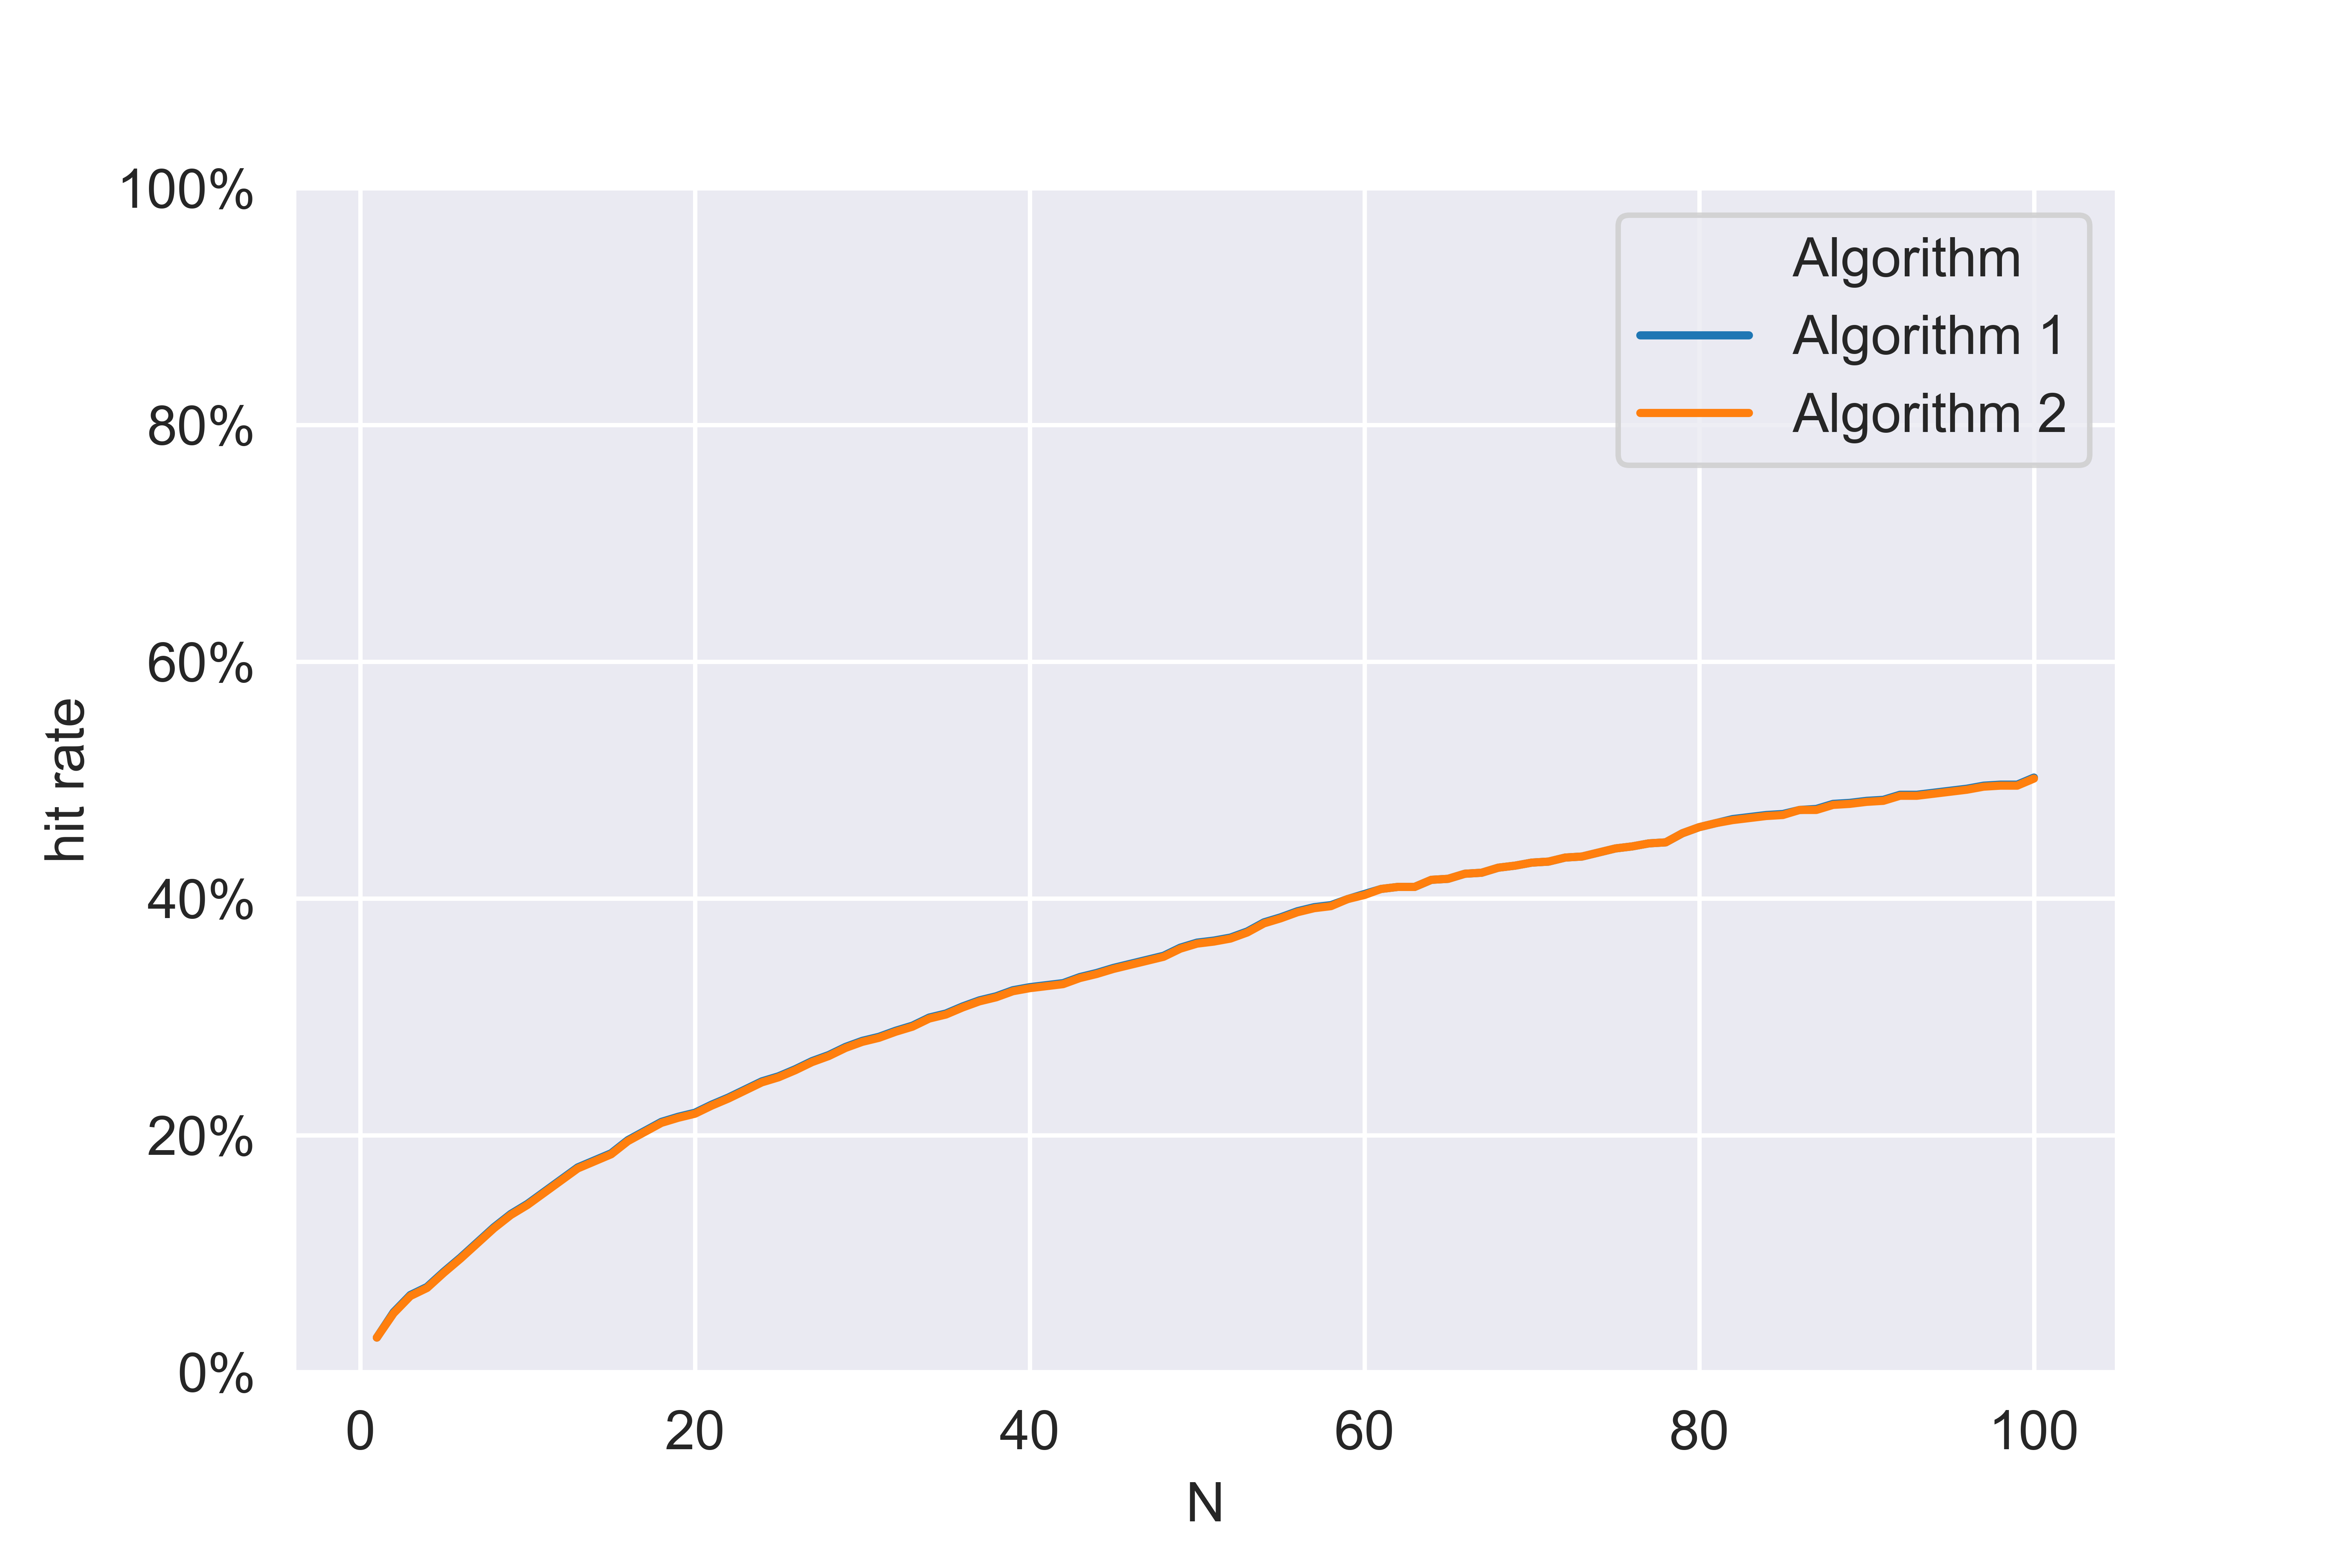
\includegraphics[width=1\linewidth]{images/fb/hit_rates_d-2.png}
        \caption{$D=2$ on linear $N$-axis.}
        \label{fig:fb_hit_rates_d2}
    \end{subfigure}%

    % d4
    \begin{subfigure}{.48\textwidth}
        \centering
        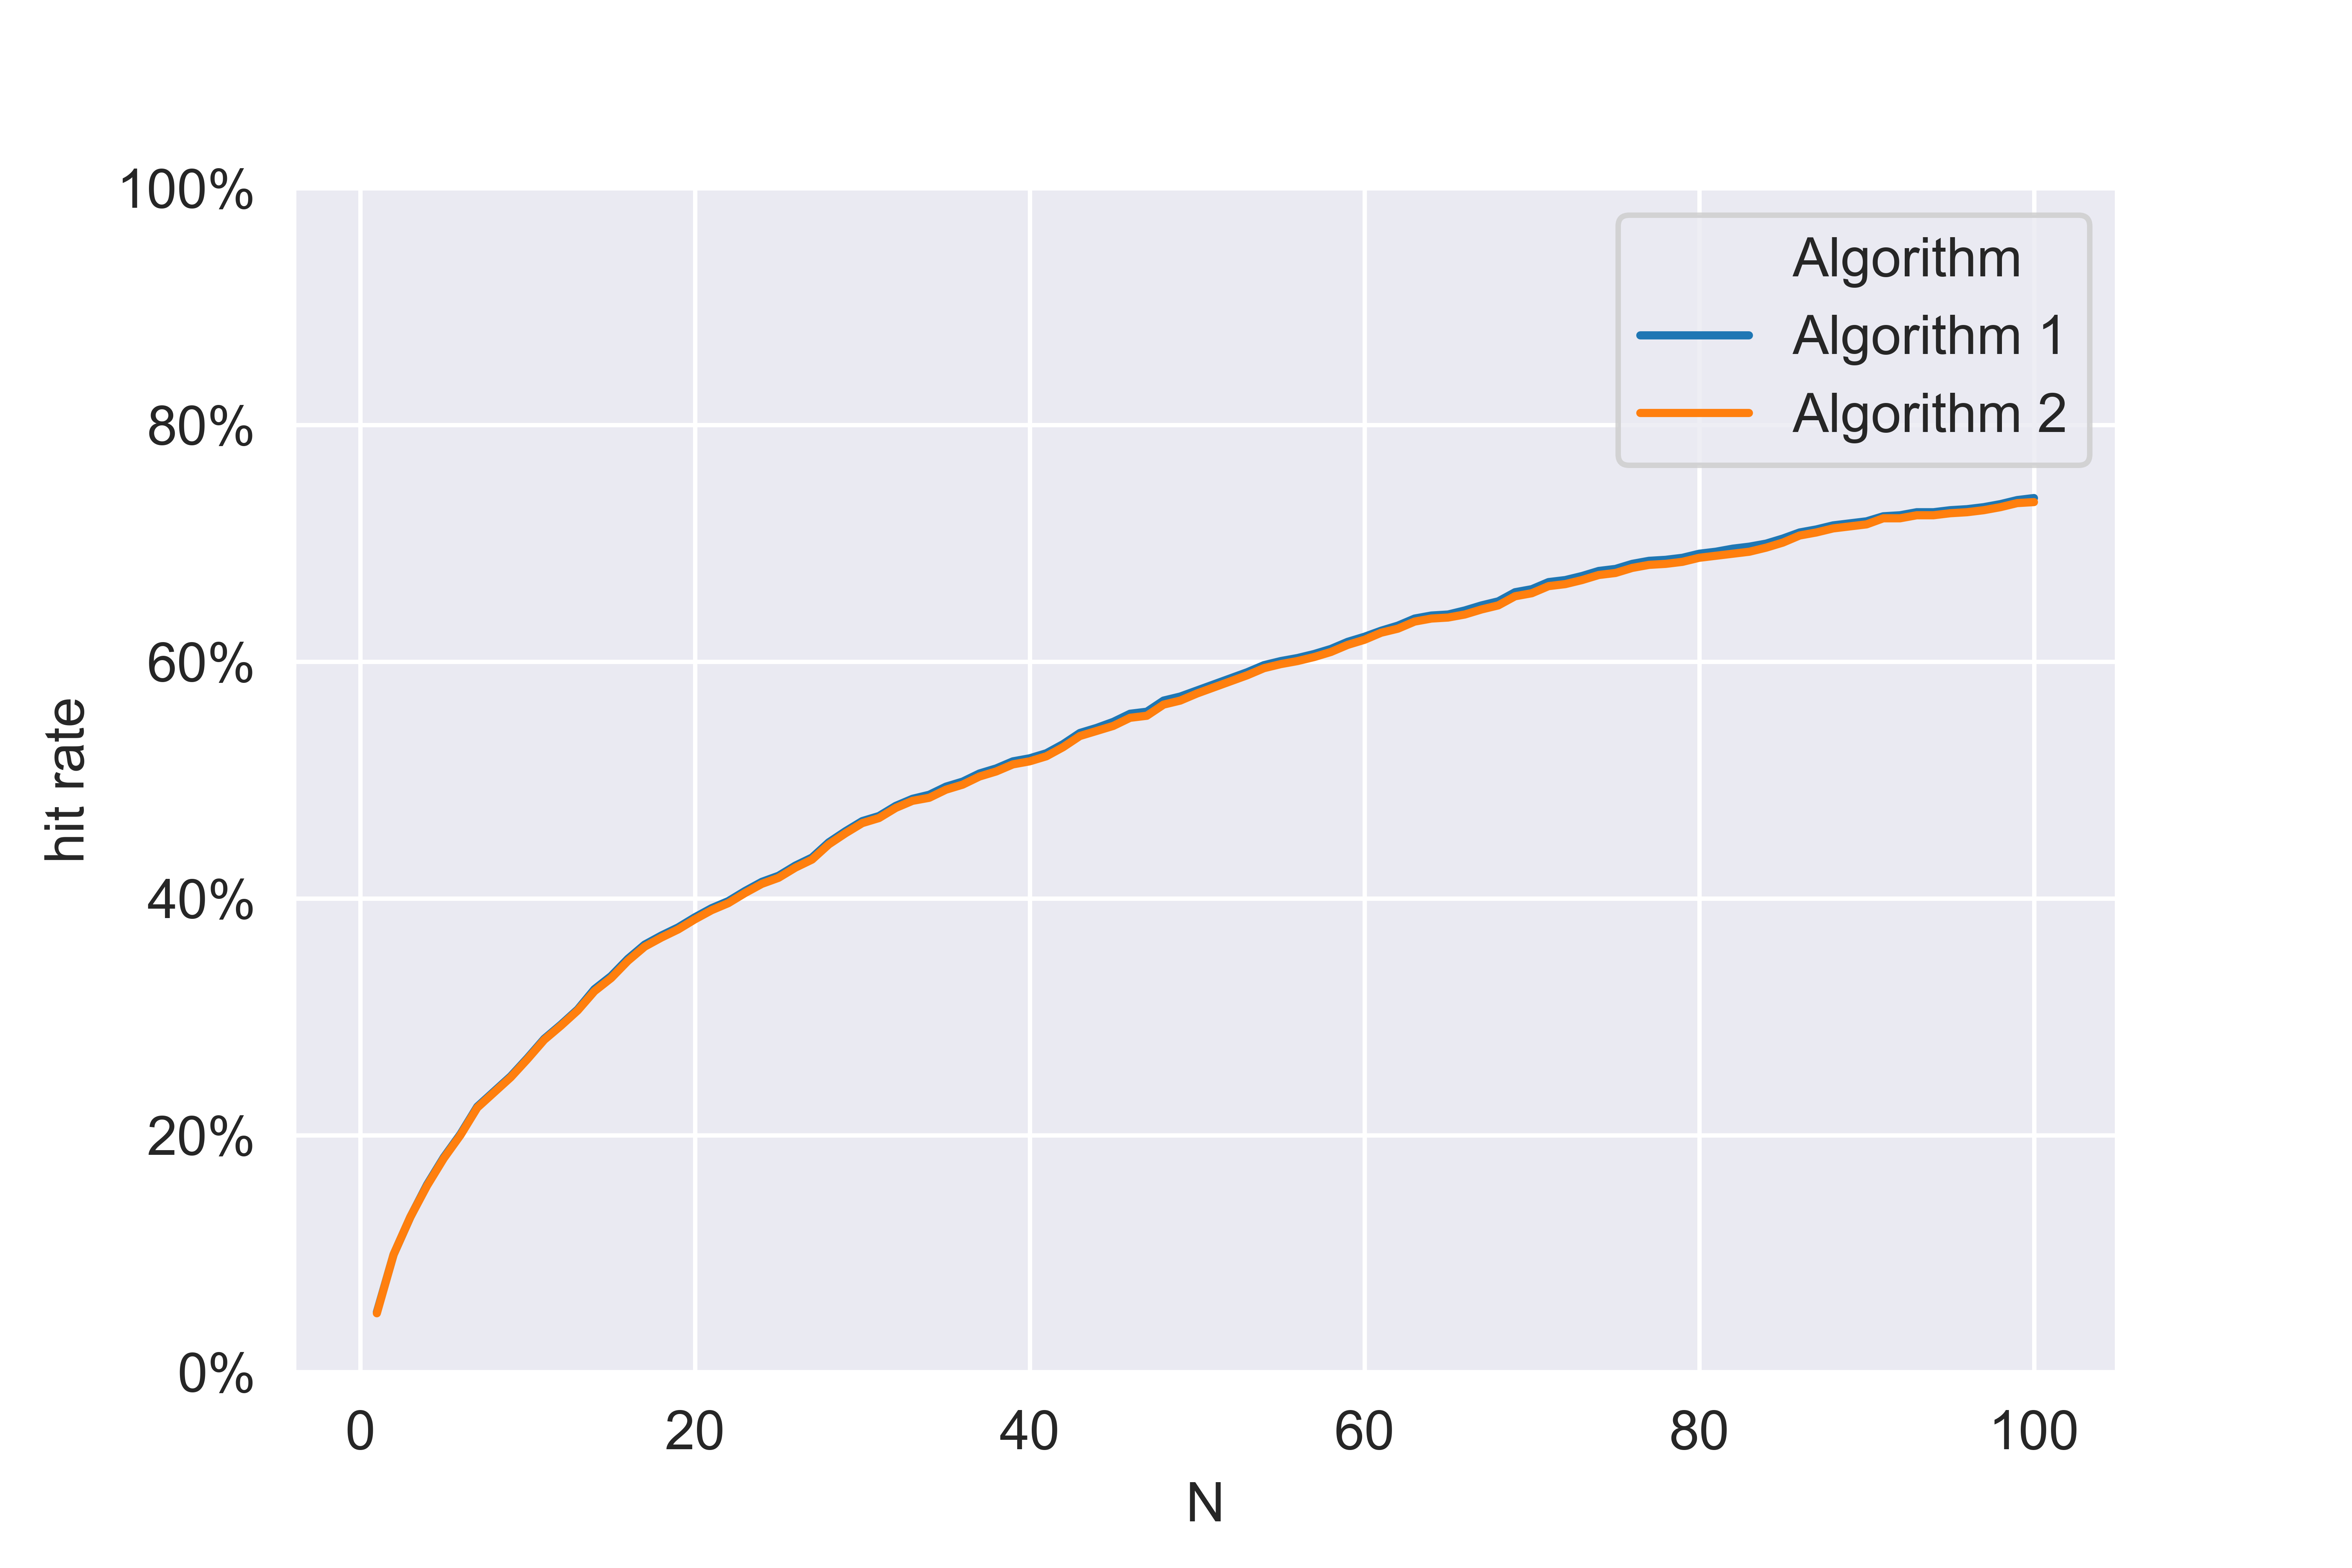
\includegraphics[width=1\linewidth]{images/fb/hit_rates_d-4.png}
        \caption{$D=4$ on linear $N$-axis.}
        \label{fig:fb_hit_rates_d4}
    \end{subfigure}%

    % d128
    \begin{subfigure}{.48\textwidth}
        \centering
        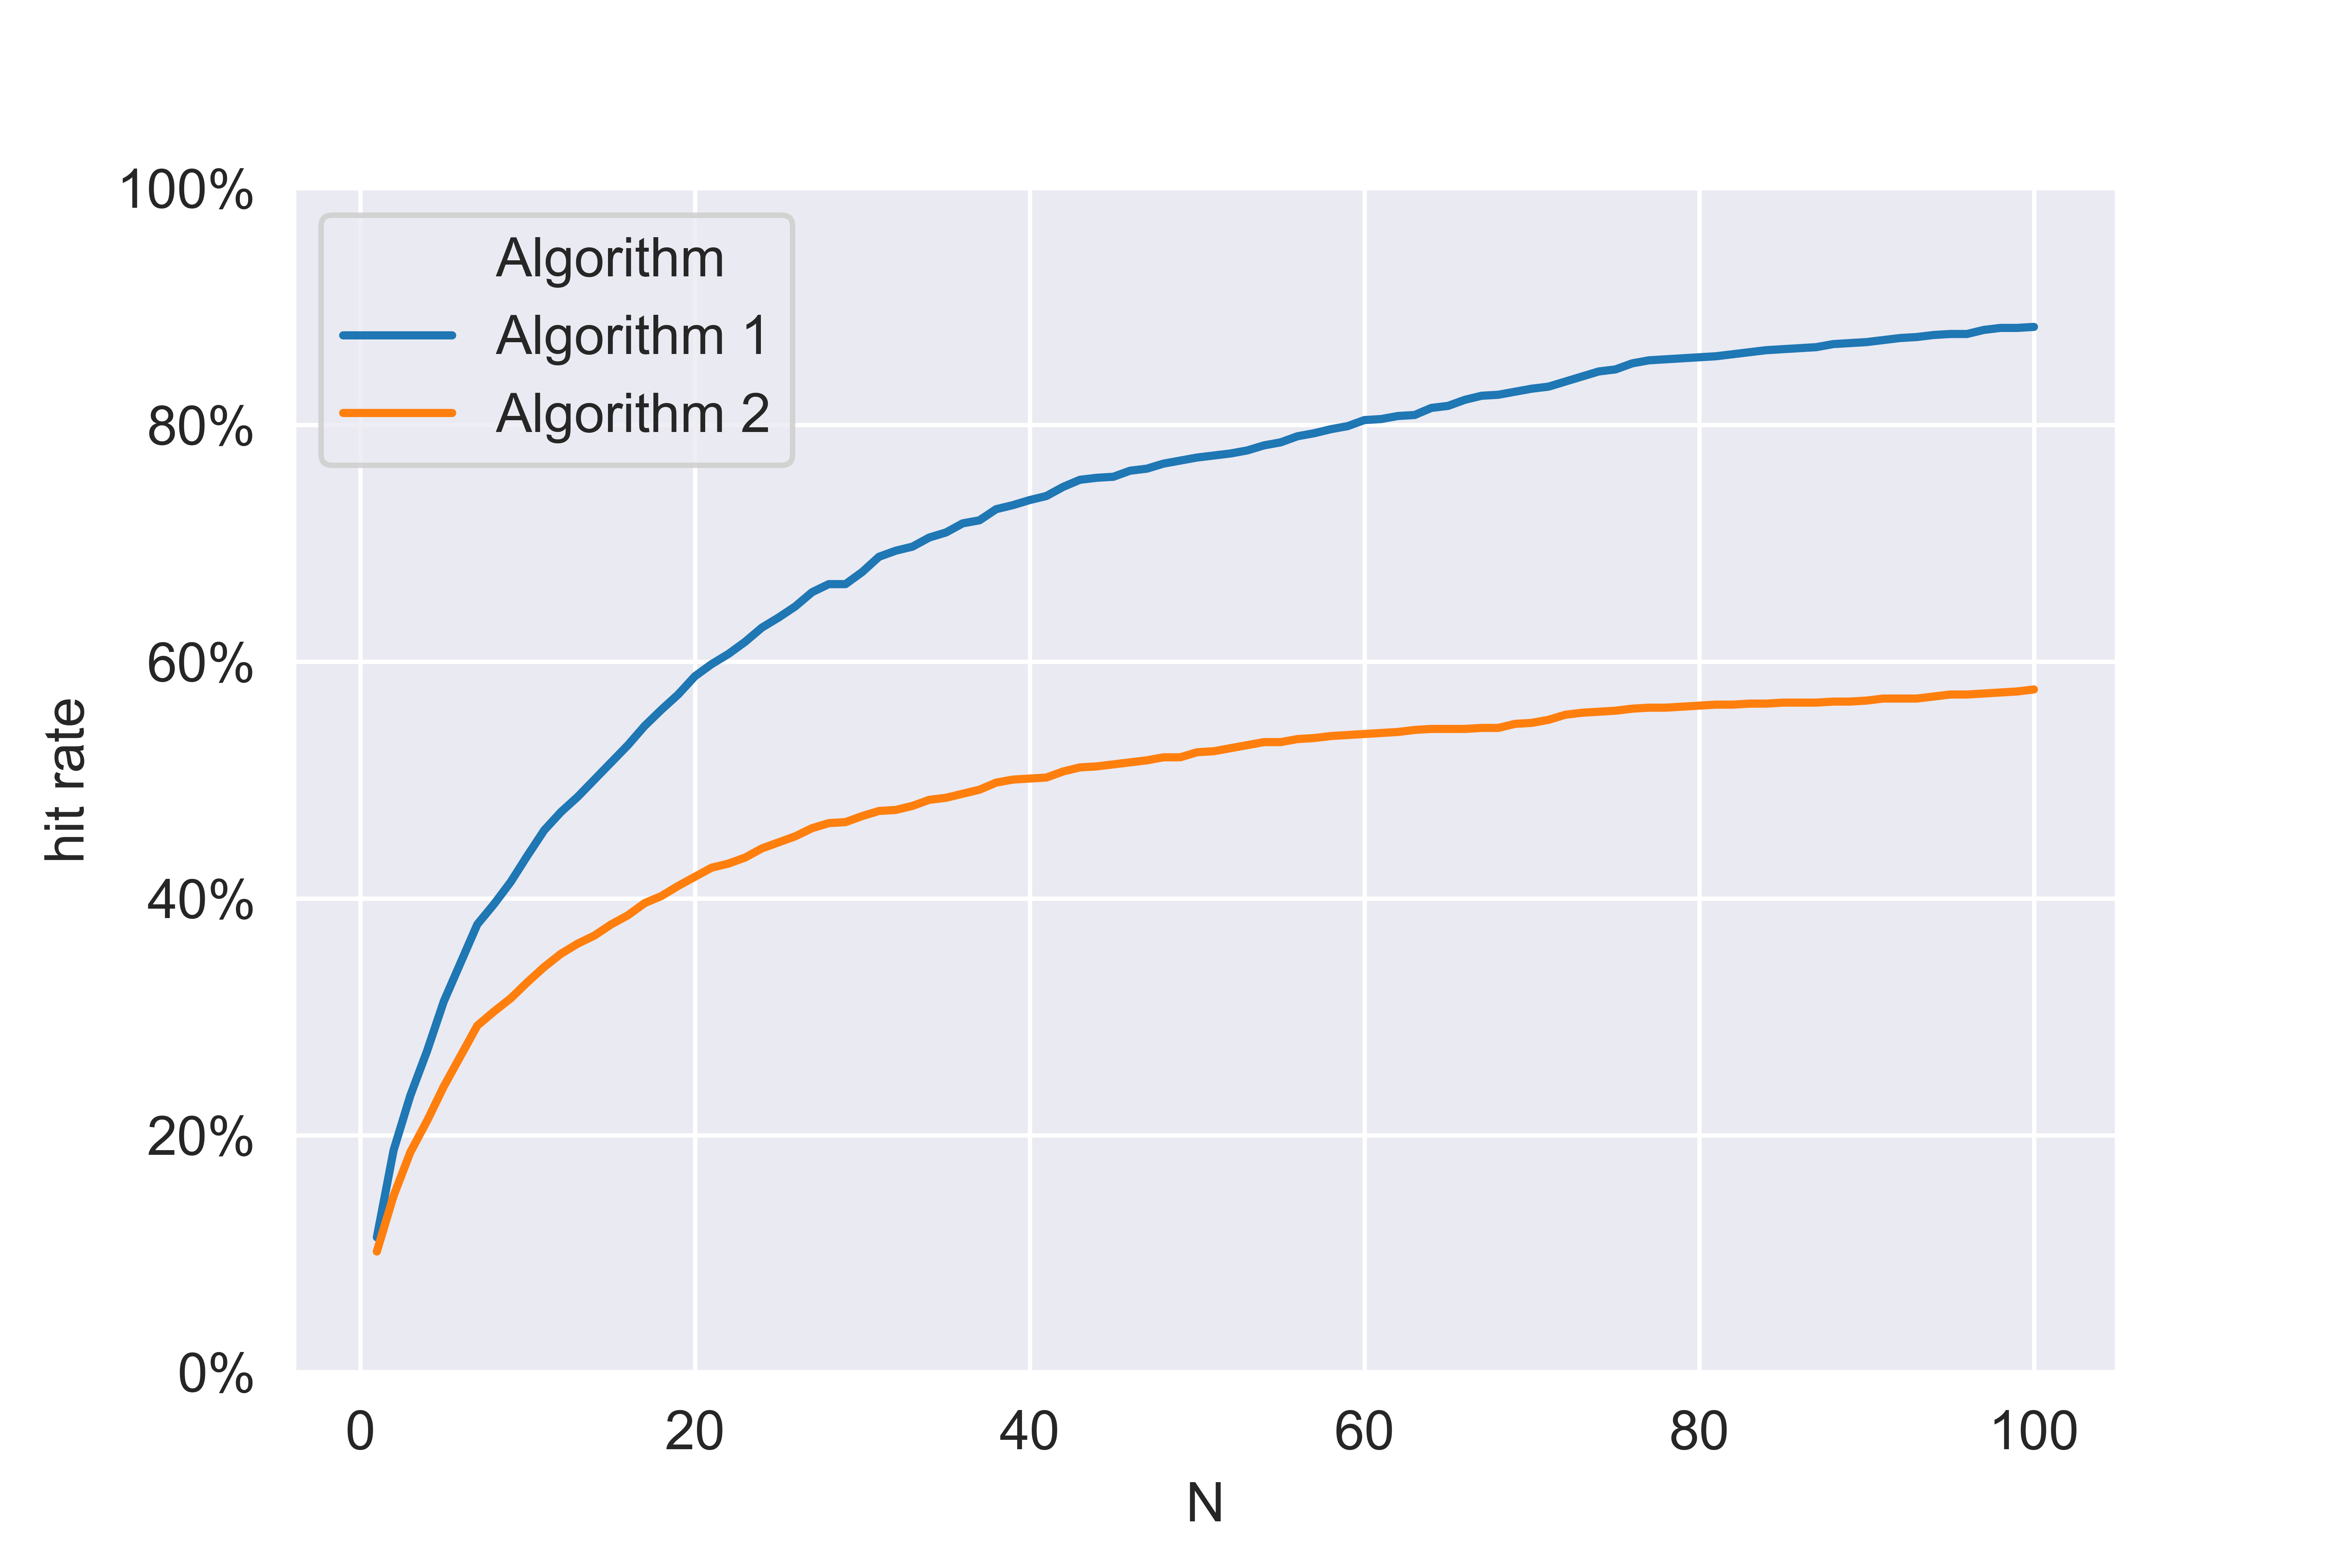
\includegraphics[width=1\linewidth]{images/fb/hit_rates_d-128.png}
        \caption{$D=128$ on linear $N$-axis.}
        \label{fig:fb_hit_rates_d128}
    \end{subfigure}%

    \caption{Hit-rates of \citetitle{social_circles_fb} graph's top-$N$ friend suggestions on $N$-axis for $D \in [2,4,128]$. Hit-rate lines for Algorithm \ref{alg:friend_sug} and Algorithm \ref{alg:friend_sug_com} overlap for $D=2$ and $D=4$.}
    \label{fig:fb_hit_rates}
\end{figure}

Two hit-rate lines are shown for each embedding representation size $D \in [2,4,128]$ on $N$-axis. The blue line shows the hit-rates when generating friend suggestions from all users (Algorithm \ref{alg:friend_sug}). The orange line shows the hit-rate when generating recommendations from users in the same community (Algorithm \ref{alg:friend_sug_com}). For lower-dimensional embeddings with $D \in [2,4]$, the hit-rates for Algorithm \ref{alg:friend_sug} and Algorithm \ref{alg:friend_sug_com} largely overlap.

Table \ref{table:fb_hit_rates} shows readings of hit-rates over the algorithms and embedding dimensionality for top-$5$, top-$10$, and top-$20$ recommendations:

\begin{figure}[h]
    \centering
    \caption{Hit-rates of \citetitle{social_circles_fb} graph's top-$N$ friend suggestions for algorithms \ref{alg:friend_sug} and \ref{alg:friend_sug_com}, $N \in [10, 20]$, and $D \in [2,4,128]$.}
    \label{table:fb_hit_rates}
    \begin{tabular}{ l | l | c | c | c }
        \hline
        \empty                                              & \empty  & top-$5$         & top-$10$        & top-$20$        \\
        \hline
        \hline
        \multirow{3}{*}{Algorithm \ref{alg:friend_sug}}     & $D=2$   & 8.5\%           & 14.2\%          & 21.9\%          \\
                                                            & $D=4$   & 18.1\%          & 26.5\%          & 38.4\%          \\
                                                            & $D=128$ & \textbf{31.3\%} & \textbf{43.6\%} & \textbf{58.8\%} \\
        \hline
        \multirow{3}{*}{Algorithm \ref{alg:friend_sug_com}} & $D=2$   & 8.4\%           & 14.1\%          & 21.8\%          \\
                                                            & $D=4$   & 18.0\%          & 26.4\%          & 38.2\%          \\
                                                            & $D=128$ & \textbf{24.1\%} & \textbf{32.9\%} & \textbf{41.8\%} \\
        \hline
    \end{tabular}
\end{figure}

Hit-rates based on top-$5$, top-$10$, and top-$20$ recommendations are chosen since higher $N$ are not practical for recommendations.

Presenting only the top-$10$ friend suggestions to users, a hit-rate of $43.6\%$ when considering all users, or $32.9\%$, when considering only users from the same community, is achieved. A top-$5$ hit-rate of $31.3\%$ (all users) and $24.1\%$ (same community) is achieved, which can be considered viable for business use-cases, especially for only showing 5 recommendations to users. A top-$20$ hit-rate of $58.8\%$ (all users) and $41.8\%$ (same community) adds to the presented results.


\section{Conclusion}

The proposed shortest-embedding-distance friend suggestion recommender system based on embeddings generated with the community embeddings algorithm ComE BGMM+VI shows promising results.
A top-$10$ recommendations hit-rate of $43.6\%$ when considering all users (Algorithm \ref{alg:friend_sug}), and over $32.9\%$ when considering users in the same community (Algorithm \ref{alg:friend_sug_com}) is achieved for Facebook friend suggestions.

\subsection{Future Work}

This work explores generating friend suggestions from node and community embeddings generated by ComE. Three values of the representation size $D$ were used in experimentation. Experimenting with more, different combinations of hyperparameters, and especially varying the number of communities $K$ might be of interest. Since in this paper, friend suggestions were explored, it is left for future work to explore item-based recommendations using embeddings. More community-centric recommendations, which deeply consider the community embeddings in generating recommendations, are left for future work.


%%% Bibliography
\printbibliography

\end{document}
